\documentclass[conference]{IEEEtran}
\IEEEoverridecommandlockouts
% The preceding line is only needed to identify funding in the first footnote. If that is unneeded, please comment it out.
\usepackage{cite}
\usepackage{amsmath,amssymb,amsfonts}
\usepackage{algorithmic}
\usepackage{graphicx}
\usepackage{textcomp}
\usepackage{xcolor}
\def\BibTeX{{\rm B\kern-.05em{\sc i\kern-.025em b}\kern-.08em
    T\kern-.1667em\lower.7ex\hbox{E}\kern-.125emX}}
\begin{document}

\title{Pilot Study on LLM-based Behavior Tree Generation:
Towards Game Character AI Creation via Natural Language}

\author{
anonymous authors
}
% \author{
% \IEEEauthorblockN{Ray Ito}
% \IEEEauthorblockA{
% \textit{Graduate School of Interdisciplinary}\\
% \textit{Information Studies}\\
% \textit{The University of Tokyo}\\
% Tokyo, Japan\\
% https://orcid.org/0009-0001-7627-8178
% }
% \and
% \IEEEauthorblockN{Naoyuki Jimbo}
% \IEEEauthorblockA{
% \textit{CyberAgent, Inc.}\\
% Tokyo, Japan
% }
% \and
% \IEEEauthorblockN{Koya Ihara}
% \IEEEauthorblockA{
% \textit{CyberAgent, Inc.}\\
% Tokyo, Japan
% }
% }

\maketitle

\begin{abstract}
Since behavior trees in modern video games require manual composition of predefined abundant nodes, designing and creating a behavior tree requires not a few work hours. Therefore, behavior tree creation assistance by large language models (LLMs) agents is likely to be significantly helpful for game designers. This paper aims to conceptualize the requirements for behavior tree creation assistance instructed by natural language, and observe the creation results with a simple agentic implementation. We categorized the requirements into four abstraction levels, ranging from direct structural descriptions to abstract design delegation, and evaluated the agent's performance in a competitive dodgeball game environment. The experimental results demonstrated that the LLM agent could accurately generate behavior tree structures when given isomorphic, detailed prompts. However, performance declined with more abstract instructions, where the agent struggled with game state management and logical node composition. These findings suggest that while LLMs possess high potential for translating natural language into behavior tree syntax, but required more appropriate context provision for adaptive creation.
\end{abstract}

\begin{IEEEkeywords}
behavior tree, large language model, game AI, non-player character, natural language processing
\end{IEEEkeywords}

\section{Introduction}

Non-player characters (NPCs) play an important role in delivering rich gameplay experiences in modern video games, one of the major contemporary entertainment forms. Behavior trees are widely adopted in the game industry as a framework for implementing NPC behavior~\cite{rabin2013game}.

While the advantage of behavior trees lies in their ability to let game designers fully specify all NPC behaviors, implementing complex NPC behavior introduces a practical bottleneck that requires significant development effort. Creating a behavior tree first requires implementing, typically through programming, all nodes representing actions and conditional branches, and then manually composing those nodes into a tree structure that precisely expresses every detail of the NPC's behavior. Since game design is an iterative activity involving repeated cycles of prototyping and playtesting~\cite{gamedesign_iterative}, behavior tree structures must be edited many times. Each editing session itself requires understanding the current tree structure and identifying locations for modification, with effort per session growing as the tree becomes larger.

To reduce this workload, this study investigates an approach in which an LLM (Large Language Model) agent is instructed via natural language to assist in generating and editing behavior trees. Recent software development practice has reported natural language-based code generation and editing workflows~\cite{vibecoding_practice}, and the ultimate goal of this study is to extend a similar framework to behavior tree authoring support, enabling game designers to rapidly implement and adjust NPC behavior.

Behavior trees have also been systematized in robotics as a hierarchical control representation~\cite{bt_survey}, and research on using LLMs to convert natural language task instructions into hierarchical structures has been reported~\cite{Izzo2024-wv,Ao2025-gl}. These approaches are characterized by transforming procedures or goals provided in natural language into the conditional-branch and action-hierarchy format of a behavior tree. The reason LLMs function effectively in robotics is that world knowledge acquired through pre-training contributes to instruction understanding and task decomposition, and external information such as skill sets, observations, and states makes it easier to ``ground'' actions~\cite{Ichter2023-jf}. In video games, however, title-specific rules, mechanics, and execution semantics are dominant, and the grounding mapping is non-trivial, making pre-training knowledge alone insufficient.

This study organizes requirements according to the abstraction level of natural language instructions into four levels, and observes how stably behavior tree generation proceeds with a standard LLM agent implementation in a competitive game environment. This paper focuses on new behavior tree generation using existing nodes and identifies state management and logical composition as primary challenges arising with increasing abstraction.

\section{Problem Formulation}

The problem addressed in this study is to interpret a designer's natural language authoring instructions via an LLM and produce or edit actual behavior tree data. While it is desirable that the LLM autonomously implement newly required nodes in the future, this paper focuses on the task of composing existing nodes---a task that falls within the designer's role.%
\footnote{In many game development studios, the workflow is divided such that programmers prepare nodes and designers compose those nodes to construct the behavior tree.}
Two scenarios can be considered in terms of when assistance is provided: generating a new behavior tree from a designer's instructions, or editing an existing behavior tree according to instructions. While the latter will be critically important in the future, this paper focuses on the former---generating new behavior trees.

The difficulty and appropriate evaluation methodology for behavior tree authoring prompts are expected to vary significantly depending on their abstraction level, i.e., the degree to which specific behaviors are detailed. We define a four-level classification in which Level~1 represents the most concrete case---essentially verbatim translation---and Level~4 represents the case most dependent on the LLM's design sensibility. This classification aims to qualitatively categorize the capabilities required of, and to be evaluated in, the LLM.

\vskip.5\baselineskip
\noindent\textbf{Implementation Delegation}: Prompts in which the designer specifies all behaviors explicitly and delegates only their implementation to the LLM.
\begin{itemize}
    \item \textbf{Level 1: Isomorphic Structured Text}\\
    A prompt in which the designer describes a tree structure isomorphic%
    \footnote{Isomorphic here means that the two tree structures agree in the number and types of nodes, the degree of each node, and all connectivity.}
    to the target behavior tree using bullet points or similar notation. The LLM agent is required to perform a verbatim translation.

    \item \textbf{Level 2: Procedural Description}\\
    A prompt in which the designer writes out procedural statements of the form ``if CONDITION, perform ACTION,'' where CONDITION and ACTION are restricted to those expressible solely by condition nodes and action nodes, respectively. The LLM is required to correctly integrate the logical relationships among multiple procedures and ensure global consistency.\\
    \textit{Example}: ``If holding 4 balls, run toward the enemy while facing them until the distance reaches 0.7; upon reaching 0.7, throw all balls; then run backward until the distance reaches 5.0.''
\end{itemize}

\noindent\textbf{Design Delegation}: Prompts in which the designer delegates part or all of the design to the LLM.
\begin{itemize}
    \item \textbf{Level 3: Partial Design Delegation}\\
    A prompt in which the designer specifies the overall behavioral goal abstractly while delegating the concrete detailed design. The LLM is required to interpret abstract instructions and concretize them as a behavior tree.\\
    \textit{Example}: ``Implement a hit-and-away tactic: approach the enemy when holding many balls, throw all of them, then retreat.''

    \item \textbf{Level 4: Full Design Delegation}\\
    A prompt in which the designer specifies a character trait without specifying behaviors and delegates the design of the entire structure. The LLM agent is required not only to construct a correctly functioning behavior tree but also to exhibit a design sensibility that expresses the specified trait.\\
    \textit{Example}: ``Create an agile NPC.''
\end{itemize}

It should be noted that the above level classification is not defined to be strictly mutually exclusive and collectively exhaustive; rather, it proposes a set of research achievement indicators based on anticipated prompts. For instance, a single prompt may contain descriptions corresponding to different levels.

\section{Experiments with a Simple Implementation}

This paper reports experiments conducted to assess the LLM's ability to understand video game context and to generate behavior trees under current conditions. These experiments correspond to the scenario of generating new behavior trees from existing nodes.

\subsection{Experimental Setup}

\subsubsection{Target Video Game}

\begin{figure}[tbp]
    \centering
    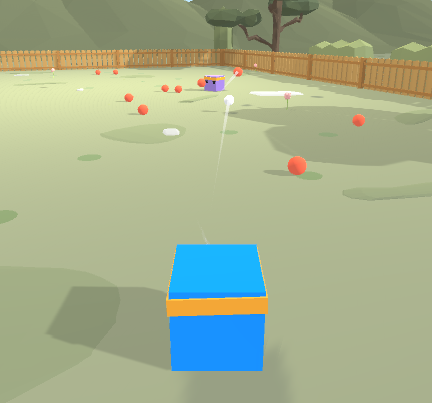
\includegraphics[width=0.8\linewidth]{image.png}
    \caption{Screenshot of the dodgeball game environment used in this study.}
    \label{fig:game}
\end{figure}

We integrated a behavior tree system into \textit{ml-agents-dodgeball-env}, a dodgeball game environment released by Unity Technologies as a reinforcement learning environment, and prepared the various nodes required for the experiment.

To simplify the requirements for NPC behavior, we removed obstacles from the game space and changed the original 4-vs-4 format to 1-vs-1 (a behavior tree agent versus a reinforcement learning model%
\footnote{We used the model specified as default in the same repository by Unity Technologies.}%
), as shown in Fig.~\ref{fig:game}.

\subsubsection{Behavior Tree System Specification}

Since behavior tree specifications are not defined uniformly and vary widely~\cite{bt_survey}, we explicitly state the specification of the behavior tree system used in this study.

The behavior tree used evaluates conditions from the root node at every game frame and selects the action node corresponding to the current game state. Only Sequence nodes maintain control state across frames. A Sequence node retains which child node it last executed; if the same Sequence node is selected in the subsequent frame, execution continues from that state. If the same Sequence node is not selected in the subsequent frame, its sequential state is reset. If condition evaluation selects no action node across the entire behavior tree, no behavior is triggered in that frame.

Instead of the behavior tree maintaining state, the in-game agent itself maintains state. For example, if the behavior tree instructs the agent to begin running in a particular direction, the agent retains that running state and direction until the behavior tree instructs it to stop.

These specifications and the types of implemented nodes were agreed upon with game developers who use behavior trees in actual production environments.

\subsubsection{LLM Agent Specification}

Since this study aims to establish a baseline for behavior tree authoring assistance technology, the implemented LLM agent is kept simple and standard. The LangGraph framework was used for implementation. The tools provided to the LLM agent were: enumeration of C\# filenames in the Unity project, reading the contents of specified C\# files, reading and writing a freely editable text file accessible across all C\# files, reading and writing behavior tree JSON files, and a function for performing static syntax analysis of those JSON files. The LLM agent was forced to continue reasoning until no errors were detected by static analysis of the behavior tree JSON. Two large language models were evaluated under identical agent configurations: the OpenAI model \texttt{gpt-5.2-2025-12-11} and the Anthropic model \texttt{claude-sonnet-4-6}.

\subsection{Prompt Level 1: Exact Match Evaluation}

By the definition of prompt Level~1, the correspondence of the behavior tree output is deterministic; the LLM agent can therefore be evaluated by its exact match rate.

\subsubsection{Method}

\begin{table}[tbp]
    \centering
    \caption{Number of Nodes in Tasks Used in the Level~1 Experiment}
    \scalebox{0.92}{
    \begin{tabular}{c|cccccccccc}
    \hline
    Task No.      & 1 & 2 &  3 & 4 & 5  &  6 &  7 &  8 &  9 & 10 \\
    \hline
    No.\ of Nodes & 5 & 4 & 10 & 8 & 11 & 23 & 14 & 14 & 14 & 12 \\
    \hline
    \end{tabular}
    }
    \label{tab:level1_nodes}
\end{table}

We prepared 10 prompt sets, each comprising a target behavior tree, the instruction ``Implement the behavior tree identical with the structure below:'', and a Markdown-format description isomorphic to the target behavior tree. The node counts of each target behavior tree are shown in Table~\ref{tab:level1_nodes}.

We computed the rate at which the JSON structure generated by the LLM agent from each prompt was actually isomorphic to the target JSON. For each of the 10 prompts, the LLM agent was executed 10 times with temperature set to 1.0, each time producing a new behavior tree JSON file from scratch.

\subsubsection{Results}

All 100 JSON structures generated by each model were isomorphic to the respective target behavior tree, yielding a perfect exact-match rate for both \texttt{gpt-5.2-2025-12-11} and \texttt{claude-sonnet-4-6}. This confirms that both models possess the ability to understand behavior tree node implementations from the codebase and to perform verbatim translation from a given prompt without any special technique.

\subsection{Prompt Level 2: Human Evaluation of Behavior}

At prompt Level~2, the behavior tree structure is not uniquely determined from the prompt; multiple behavior tree representations that correctly realize the same prompt are conceivable. We therefore evaluated behavior visually based on actual game execution.

\subsubsection{Method}

For each of the 10 behavior trees used in Level~1, we decomposed the behavior into procedural statements of the form ``if CONDITION, then ACTION.'' Where priorities were required among procedures%
\footnote{This applies when the condition statements of multiple procedures are not mutually exclusive.}%
, we added priority statements such as ``Prioritize A more than B.'' To examine whether the LLM could correctly integrate each procedure, we prepared up to four prompts per behavior tree with the statement order randomly shuffled%
\footnote{Tasks with only 1 or 2 statements produced only 1 or 2 prompts, respectively.}%
.

For each prompt, with temperature set to 0.0, each LLM agent independently generated a behavior tree. Each behavior tree was executed in the game, and the authors visually evaluated whether each procedure achieved the specified behavior under the specified conditions.

\subsubsection{Results}

\begin{table*}[tbp]
\centering
\caption{Level~2 Experimental Results (SR = Success Rate)}\label{tab:level2}
\begin{tabular}{c|cccccccccc}
\hline
Task No.                     &  1            &  2            &  3            &  4            &  5   &  6  &  7            &  8   &  9            & 10            \\
\hline
No.\ of Procedures           &  1            &  2            &  3            &  2            &  4   &  3  &  5            &  5   &  6            &  5            \\
SR (\texttt{gpt-5.2})        & \textbf{1.0} & \textbf{1.0} & \textbf{1.0} & \textbf{1.0} & 0.75 & 0.0 & \textbf{1.0} & 0.25 & \textbf{1.0} & \textbf{1.0} \\
SR (\texttt{claude-sonnet-4-6}) & \textbf{1.0} & \textbf{1.0} & \textbf{1.0} & \textbf{1.0} & 0.75 & 0.0 & \textbf{1.0} & 0.25 & \textbf{1.0} & \textbf{1.0} \\
\hline
\end{tabular}
\end{table*}

The results are shown in Table~\ref{tab:level2}.%
\footnote{Success was defined as confirming that all procedural descriptions were realized.}
Both models achieved a success rate of 1.0 in 7 out of 10 tasks, and both exhibited failures exclusively in Tasks~5, 6, and 8.

In Task~5, one run per model produced a behavior tree consisting solely of condition nodes with no action nodes. Since the JSON structure was syntactically valid, it passed static analysis. This is likely attributable to the LLM agent deciding to abort generation partway through.

In Task~6, all failure cases across both models shared a common inability to correctly express the following as behavior: ``If you can see the enemy, keep looking at the enemy and strafing. Strafing is to move left, forward, right, back 0.5 seconds each.'' Because the behavior tree system does not maintain state within the tree itself, placing a ``run left for 0.5 seconds'' action node immediately before an unconditional ``run forward for 0.5 seconds'' action node under a Sequence node causes the latter to execute in the very next frame. A condition confirming that the preceding leftward run has lasted 0.5 seconds must therefore be incorporated. All failure cases in this task resulted from omitting this timing condition management.

In Task~8, the three failure cases per model exhibited a situation in which the procedure ``if a dropped ball is visible and not holding more than 3 balls, run to the ball'' failed to stop a rotation state initiated by a different procedure, preventing the agent from successfully running toward the ball. In other tasks, ball-collection behavior was either described as ``look and go to the ball,'' which implicitly overrides rotation, or rotation was never instructed throughout (Task~2), so this issue did not arise. In the one success case per model, the rotation was correctly stopped. While it is practically expected that each procedure is expressed without gaps when composing multiple procedures, these results suggest that both models' abilities to accurately anticipate game state management during authoring are still developing.

Notably, the success rates for \texttt{gpt-5.2-2025-12-11} and \texttt{claude-sonnet-4-6} were identical across all tasks. This agreement between two independently developed models suggests that the observed failures are attributable to the inherent difficulty of timing and state management in this game environment, rather than to model-specific limitations.

\subsection{Prompt Level 4: Win Rate Evaluation}

For prompt Levels~3 and 4, the LLM agent is given significant discretion regarding how to realize the behavior, and evaluation methodology requires careful design. In this paper, we evaluate Level~4 by computing a simple ``strength'' metric to assess whether the LLM agent can autonomously compose a behavior tree appropriately suited to the game.

\subsubsection{Method}

We prepared 10 prompts requesting maximum combat performance, such as ``Create a powerful player that never loses,'' and for each prompt had each LLM agent independently generate three behavior trees with temperature set to 1.0, yielding 30 behavior trees per model.

Each behavior tree-driven agent played 10 matches against the reinforcement learning agent, and the simple win rate was computed.

\subsubsection{Results}

\begin{figure}[tbp]
    \centering
    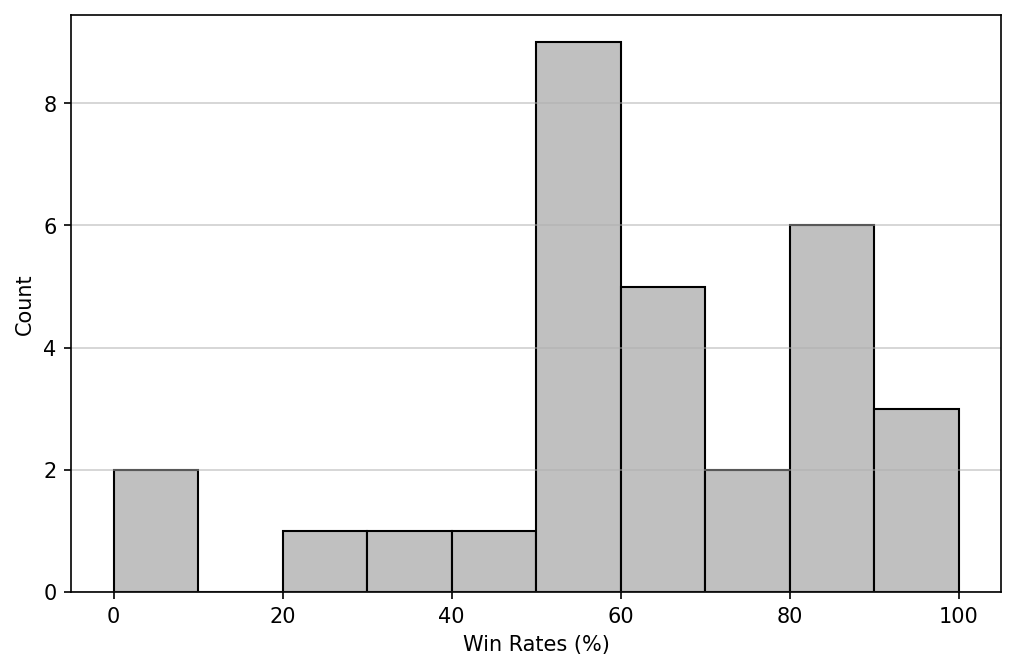
\includegraphics[width=0.48\linewidth]{winrate.png}
    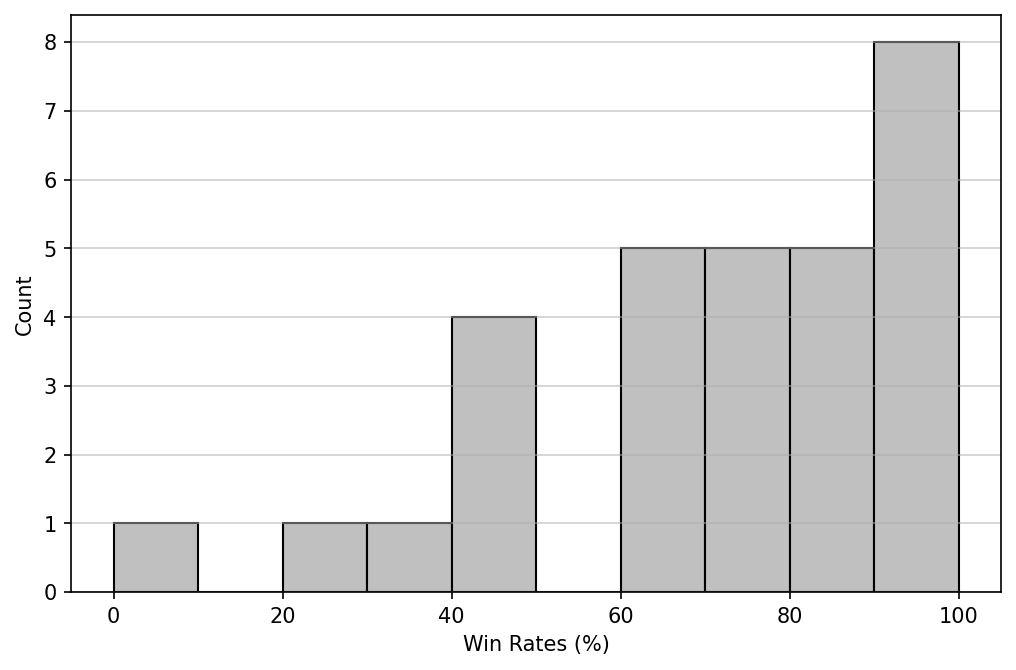
\includegraphics[width=0.48\linewidth]{winrate_claude.png}
    \caption{Histograms of win rates in the Level~4 experiment for \texttt{gpt-5.2-2025-12-11} (left) and \texttt{claude-sonnet-4-6} (right).}
    \label{fig:level4}
\end{figure}

The win rates for each prompt are summarized in the histograms shown in Fig.~\ref{fig:level4}. For \texttt{gpt-5.2-2025-12-11}, the mean win rate was 58.0\% and the median was 60.0\%. For \texttt{claude-sonnet-4-6}, the mean win rate was 67.3\% and the median was 70.0\%. Both distributions span from 0\% to 100\%, and both models exhibited a tendency to outperform the reinforcement learning baseline; \texttt{claude-sonnet-4-6} showed a higher central tendency than \texttt{gpt-5.2-2025-12-11}.

For \texttt{gpt-5.2-2025-12-11}, the two cases with a 0\% win rate both showed agents that barely moved during gameplay. In one case, two independent nodes---``if the enemy is visible, look toward the enemy'' and ``if the enemy is visible, approach the enemy''---were both connected under the root Selector node. Due to the semantics of the Selector node, only the former was ever executed, causing the agent to do nothing but face the enemy. For \texttt{claude-sonnet-4-6}, one case with a 0\% win rate was similarly observed, also resulting in near-complete agent inactivity. These cases demonstrate that both models can fail to correctly apply control node semantics despite having direct access to their implementation code.

\section{Conclusion}

In this paper, we organized requirements for behavior tree authoring support via natural language instructions into four abstraction levels and conducted a baseline observation with a standard LLM agent implementation. Level~1 (isomorphic structured text) yielded perfect correspondence with the target behavior tree, confirming that current LLMs possess the ability to perform verbatim mapping to behavior tree syntax. In contrast, more abstract instructions (Level~2 and above) led to reduced success rates, with state management in time-driven game execution (timing conditions and action overriding) and logical integration of multiple procedures (appropriate construction of conditional branches and priority relationships) emerging as primary difficulties. In Level~4, win rates were broadly distributed from 0\% to 100\%, with cases in which misuse of control node semantics directly degraded performance.

The limitations of this paper include: (i)~the number of evaluation tasks and the scale of the behavior trees are limited and do not adequately represent the difficulty of large-scale commercial titles; (ii)~the Level~2 evaluation is primarily visual, leaving room to improve the objectivity and reproducibility of assessment; and (iii)~the LLM was not provided with information about runtime behavior, leaving it with insufficient cues to detect and correct temporal state inconsistencies in time-driven environments.

As future work, we will investigate how to present time-driven execution semantics---including state transitions, timing conditions, and action override relationships---to the LLM in order to strengthen game-context grounding. This capability serves as a foundation not only for behavior debugging toward behavior tree self-repair, but also for realizing interactive authoring support that responds to user corrections and specification changes. For time-driven environments, world model learning that captures state transitions has been proposed~\cite{ha2018world}, and observation design enabling behavior understanding based on state sequences may be key for behavior tree generation and editing. Furthermore, frameworks for incorporating and grounding title-specific rules and mechanics as external knowledge have been proposed~\cite{fan2022minedojo}, and systematically evaluating presentation methods that integrate title-specific information with runtime state information constitutes a primary avenue for future work.

\bibliographystyle{IEEEtran}
\bibliography{main}

\end{document}
